\documentclass[conference]{IEEEtran}
\IEEEoverridecommandlockouts

\usepackage{cite}
\usepackage{amsmath,amssymb,amsfonts}
\usepackage{algorithmic}
\usepackage{graphicx}
\usepackage{textcomp}
\usepackage{xcolor}
\usepackage{booktabs}
\usepackage{tabularx}
\usepackage{microtype}
\usepackage{url}
\usepackage{hyperref}
\usepackage{tikz}
\usetikzlibrary{shapes.geometric, arrows.meta, positioning, calc}

\def\BibTeX{{\rm B\kern-.05em{\sc i\kern-.025em b}\kern-.08em
    T\kern-.1667em\lower.7ex\hbox{E}\kern-.125emX}}

\begin{document}

\title{Multimodal Wearable Stress Detection: Implementation, Spatio-Temporal Graph Neural Networks, and Leave-One-Subject-Out Cross-Validation\\
\thanks{Capstone Technical Review 2, Project Group: Chota Chatri, School of Computer Science and Engineering, Vellore Institute of Technology, India.}
}

\author{
\IEEEauthorblockN{Bhavya Singh}
\IEEEauthorblockA{\textit{School of Computer Science and Eng.} \\
\textit{Vellore Institute of Technology}\\
Vellore, India \\
Reg. No: 25BCE2004}
\and
\IEEEauthorblockN{Soham Sharma}
\IEEEauthorblockA{\textit{School of Computer Science and Eng.} \\
\textit{Vellore Institute of Technology}\\
Vellore, India \\
Reg. No: 25BCE0403}
\and
\IEEEauthorblockN{Praneet Raj}
\IEEEauthorblockA{\textit{School of Computer Science and Eng.} \\
\textit{Vellore Institute of Technology}\\
Vellore, India \\
Reg. No: 25BCE2280}
}

\maketitle

\begin{abstract}
Stress is a multi-faceted psychophysiological state governed by the complex interplay between the sympathetic and parasympathetic branches of the Autonomic Nervous System (ANS). While traditional wearable stress detection approaches rely on isolated unimodal streams or handcrafted features evaluated under random train-test splits, they systematically suffer from cross-subject baseline drift and fail to model dynamic cross-channel physiological coupling. Building upon the theoretical architecture proposed in Review 1, this paper presents the complete implementation, optimization, and empirical evaluation of an end-to-end multimodal stress detection framework evaluated against the benchmark Wearable Stress and Affect Detection (WESAD) dataset. We extract, temporally calibrate, and filter three physical sensor streams---AD8232 single-lead ECG, MAX30102 PPG, and DS18B20 skin temperature---resampled to a synchronized 128~Hz timebase and segmented into 22,192 three-second sliding windows across 15 subjects. 

We systematically evaluate seven distinct architectures across both deep learning and classical paradigms: 1D-CNN, Bidirectional LSTM, Temporal Transformer, Spatio-Temporal Graph Convolutional Network (ST-GCN), Random Forest, Support Vector Machines (SVM), and XGBoost, utilizing a strict 15-fold Leave-One-Subject-Out Cross-Validation (LOSO-CV) protocol to guarantee zero data leakage across subjects. Our proposed ST-GCN models the human body as a dynamic graph topology where edge weights are formulated via per-window Pearson cross-correlation matrices between cardiac (ECG/PPG) and thermal biosignals. ST-GCN achieves champion deep learning performance with $76.50\% \pm 16.5\%$ accuracy, an F1-score of $0.6578 \pm 0.216$, and an AUC-ROC of $0.8665 \pm 0.135$, while executing single-window inference in $2.57 \pm 1.51$~ms on CPU---comfortably satisfying the hard $< 50$~ms real-time requirement for ESP32 microcontroller packet streaming. Finally, the champion model is exported to an ultra-lightweight 73.8~KB ONNX binary, validated with a numerical output deviation of only $4.768 \times 10^{-6}$ against native PyTorch, and packaged into a standalone inference engine (\texttt{inference.py}) operating without PyTorch runtime dependencies.
\end{abstract}

\begin{IEEEkeywords}
Multimodal deep learning, wearable physiological sensors, stress detection, Spatio-Temporal Graph Convolutional Networks (ST-GCN), Leave-One-Subject-Out (LOSO) cross-validation, ONNX runtime, real-time edge computing.
\end{IEEEkeywords}

\section{Introduction \& Progression from Review 1}

\subsection{Context and Review 1 Foundation}
In Review 1 (\textit{Multimodal Stress Detection System: Literature Review, Proposed Architecture, and System Design}), our team established the theoretical basis of multimodal physiological stress detection. We conducted an extensive critical survey of seven landmark works spanning acoustic analysis, unimodal physiological monitoring, and time-frequency transformations (e.g., MMFD-SD \cite{xiang2025}, MuSE \cite{bara2020}, and 2D Gramian Angular Field transforms \cite{yang2025}). The core theoretical conclusion established in Review 1 was that unimodal systems (relying solely on heart rate or electrodermal activity) are intrinsically vulnerable to motion artifacts, sensor displacement, and individual baseline variance. 

To overcome these constraints, Review 1 proposed a Graph Neural Network (GNN)-centered multimodal fusion framework, conceptualizing physiological sensors not as independent 1D time-series vectors, but as nodes within a dynamically coupled physiological graph.

\subsection{Review 2 Objectives Accomplished}
In this Review 2 milestone, we have translated the conceptual design from Review 1 into a fully realized, empirical software and model pipeline:
\begin{enumerate}
    \item \textbf{Multimodal Alignment Pipeline:} Engineered a robust signal ingestion pipeline aligning ECG, PPG, and skin temperature from raw WESAD pickle archives into synchronized 128~Hz sliding windows.
    \item \textbf{Dynamic Graph Formulation:} Implemented a vectorized, PyG-independent Spatio-Temporal Graph Convolutional Network (ST-GCN) computing dynamic Pearson correlation adjacency matrices per sample.
    \item \textbf{Rigorous Person-Independent Benchmarking:} Executed complete 15-fold Leave-One-Subject-Out Cross-Validation (LOSO-CV), preventing the optimistic over-fitting typical of random $k$-fold splits.
    \item \textbf{Hardware Latency Verification:} Measured CPU latency per 3-second window to validate compatibility with ESP32-based telemetry gateways ($< 50$~ms budget).
    \item \textbf{Edge Deployment Handoff:} Exported the optimal model to ONNX format with strict numerical equivalence testing, ready for immediate firmware integration in Review 3.
\end{enumerate}

\section{Multimodal Signal Preprocessing \& Windowing Pipeline}

\subsection{Physical Sensor to Dataset Mapping}
The target hardware platform for our capstone platform comprises an \textbf{ESP32} microcontroller interfacing with an \textbf{AD8232} ECG analog front-end, a \textbf{MAX30102} optical pulse oximetry sensor, and a \textbf{DS18B20} digital temperature probe. To train and benchmark our models prior to physical hardware fabrication, we map these exact sensor modalities to the gold-standard \textbf{WESAD} dataset \cite{schmidt2018}:

\begin{table}[htbp]
\caption{Physical Sensor to Dataset Mapping and Resampling Strategy}
\label{tab:sensor_mapping}
\centering
\footnotesize
\begin{tabularx}{\columnwidth}{@{}lXccX@{}}
\toprule
\textbf{Sensor} & \textbf{Modality} & \textbf{WESAD Source} & \textbf{Native} & \textbf{Resampling} \\
\midrule
AD8232 & Lead-I ECG & \texttt{chest['ECG']} & 700\,Hz & FIR Decimation \\
MAX30102 & PPG (BVP) & \texttt{wrist['BVP']} & 64\,Hz & Cubic Spline \\
DS18B20 & Skin Temp & \texttt{wrist['TEMP']} & 4\,Hz & Linear Interp. \\
Labels & Protocol & \texttt{chest['label']} & 700\,Hz & Mode Aggregation \\
\bottomrule
\end{tabularx}
\end{table}

\subsection{Signal Conditioning \& Filtering}
Wearable physiological signals are highly vulnerable to powerline interference, motion transients, and baseline drift. We apply a three-stage conditioning cascade in strict chronological order per subject:

\begin{enumerate}
    \item \textbf{Powerline Interference Suppression:}
    A digital 2nd-order Infinite Impulse Response (IIR) notch filter is applied across all channels at $f_0 = 50.0\text{ Hz}$ with quality factor $Q = 30.0$:
    \begin{equation}
    \omega_0 = \frac{2\pi f_0}{f_s}, \quad H(z) = \frac{1 - 2\cos(\omega_0)z^{-1} + z^{-2}}{1 - 2r\cos(\omega_0)z^{-1} + r^2 z^{-2}}
    \end{equation}
    where $r \approx 1 - \frac{\pi f_0}{Q f_s}$.

    \item \textbf{Physiological Bandpass Filtering:}
    \begin{itemize}
        \item \textbf{ECG:} 4th-order zero-phase Butterworth bandpass filter between $0.5\text{ Hz}$ (eliminating respiration baseline wander) and $40.0\text{ Hz}$ (eliminating electromyographic high-frequency noise).
        \item \textbf{PPG:} 3rd-order zero-phase Butterworth bandpass filter between $0.5\text{ Hz}$ and $5.0\text{ Hz}$ (isolating arterial pulse wave reflections while removing motion transients).
        \item \textbf{Skin Temperature:} Retains low-frequency dynamics without bandpass filtering (notch filtering only).
    \end{itemize}

    \item \textbf{Subject-Wise Z-Score Normalization:}
    To mitigate cross-subject baseline variability without leaking test-fold statistics into training sets, each subject channel $x$ is normalized independently:
    \begin{equation}
    z(t) = \frac{x(t) - \mu_{\text{subject}}}{\sigma_{\text{subject}} + \epsilon}
    \end{equation}
\end{enumerate}

\subsection{Windowing and Binary Label Formulation}
Continuous filtered signals are partitioned using a sliding window:
\begin{itemize}
    \item \textbf{Window Duration ($T_{\text{win}}$):} 3.0 seconds ($W = 384\text{ samples}$ at 128~Hz).
    \item \textbf{Overlap:} 50\% ($1.5\text{ seconds}$ step size, $\Delta W = 192\text{ samples}$).
    \item \textbf{Binary Classification Label Formulation:}
    \begin{itemize}
        \item \textbf{Class 0 (Non-Stress):} WESAD Condition 1 (Baseline cognitive state) and Condition 3 (Amusement / positive valence).
        \item \textbf{Class 1 (Acute Stress):} WESAD Condition 2 (Trier Social Stress Test --- TSST mental arithmetic and public speaking stressors).
        \item Transient segments (Conditions 0, 4, 5, 6, 7) are strictly excised.
    \end{itemize}
\end{itemize}

The compiled dataset yields $N = 22,192$ multimodal windows (tensor shape $[22192, 3, 384]$), with a global stress prevalence of 30.1\% (6,682 stress windows vs. 15,510 non-stress windows). The compiled corpus is serialized into a compressed archive (\texttt{wesad\_windows.npz}, 39.5~MB), reducing data loading time from 3 minutes to 0.2 seconds.

\subsection{Classical Feature Extraction (15 Biomarkers)}
For comparison against shallow machine learning baselines, each 3-second window is transformed into a 15-dimensional handcrafted biomarker vector:
\begin{itemize}
    \item \textbf{Cardiovascular \& HRV (ECG):} Mean RR-interval, SDNN ($\text{Std}(RR)$), RMSSD ($\sqrt{\text{Mean}(\Delta RR^2)}$), pNN50, Very Low Frequency (VLF: $0.0033–0.04\text{ Hz}$), Low Frequency (LF: $0.04–0.15\text{ Hz}$), High Frequency (HF: $0.15–0.40\text{ Hz}$), and Sympathovagal balance ($\text{LF}/\text{HF}$ ratio).
    \item \textbf{Hemodynamic Features (PPG):} Systolic peak amplitude, pulse interval variance, peak-to-peak amplitude standard deviation, and blood volume proxy.
    \item \textbf{Thermal Features (Skin Temp):} Mean window temperature, temperature variance, and thermal slope ($\Delta T / \Delta t$ reflecting peripheral vasoconstriction).
\end{itemize}

\section{Deep Learning \& Graph Architectures Implementation}

\subsection{1D-Convolutional Neural Network (1D-CNN)}
The 1D-CNN models temporal waveform morphology across channels. It comprises three sequential convolutional blocks:
\begin{itemize}
    \item Block 1: $\text{Conv1D}(c_{\text{in}}=3, c_{\text{out}}=32, k=7, s=2, p=3) \rightarrow \text{BatchNorm} \rightarrow \text{ReLU} \rightarrow \text{MaxPool}(2)$.
    \item Block 2: $\text{Conv1D}(32, 64, k=5, s=2, p=2) \rightarrow \text{BatchNorm} \rightarrow \text{ReLU} \rightarrow \text{MaxPool}(2)$.
    \item Block 3: $\text{Conv1D}(64, 128, k=3, s=1, p=1) \rightarrow \text{BatchNorm} \rightarrow \text{ReLU} \rightarrow \text{AdaptiveAvgPool1D}(1)$.
    \item Classification: Flatten $\rightarrow \text{Linear}(128, 64) \rightarrow \text{Dropout}(0.3) \rightarrow \text{Linear}(64, 2)$.
\end{itemize}

\subsection{Bidirectional LSTM (BiLSTM)}
The BiLSTM captures forward and reverse sequential dependencies. Input tensors $[B, 3, 384]$ are transposed to sequence format $[B, 384, 3]$. A 2-layer BiLSTM with hidden dimension $h=64$ processes the timesteps, producing concatenated hidden states of size 128. Global temporal average pooling followed by a dense projection yields logits:
\begin{equation}
H_t = [\overrightarrow{\text{LSTM}}(x_t); \overleftarrow{\text{LSTM}}(x_t)], \quad \bar{H} = \frac{1}{T}\sum_{t=1}^T H_t, \quad y = \text{Linear}(\bar{H})
\end{equation}

\subsection{Temporal Transformer}
The Transformer models long-range attention without recurrent bottlenecks. The 3 channels are projected to embedding dimension $d_{\text{model}} = 64$ via a 1D convolution. Sinusoidal positional encodings are summed with the embeddings. Two Transformer Encoder layers (4 attention heads, feedforward dimension 128, dropout 0.1) apply scaled dot-product attention:
\begin{equation}
\text{Attention}(Q, K, V) = \text{softmax}\left(\frac{QK^T}{\sqrt{d_k}}\right)V
\end{equation}
The sequence representation is pooled across the temporal dimension and classified via a 2-layer MLP.

\subsection{Spatio-Temporal Graph Convolutional Network (ST-GCN)}
Standard deep models treat ECG, PPG, and temperature as static isolated channels. However, psychophysiological stress responses exhibit \textbf{dynamic autonomic coupling}: sympathetic activation simultaneously accelerates heart rate (ECG R-peak shortening), induces peripheral vasoconstriction (attenuated PPG pulse amplitude), and suppresses peripheral skin perfusion (falling temperature).

To model this, we construct a 3-node graph $\mathcal{G} = (\mathcal{V}, \mathcal{E})$ for every 3-second window, where $\mathcal{V} = \{\text{ECG}, \text{PPG}, \text{Temp}\}$:

\begin{enumerate}
    \item \textbf{Dynamic Pearson Adjacency Matrix Formulation:}
    For a given sample $x \in \mathbb{R}^{3 \times T}$, we compute the zero-mean centered signal $\tilde{x} = x - \mu_x$. The empirical cross-channel correlation matrix $R \in \mathbb{R}^{3 \times 3}$ is calculated dynamically via batch matrix multiplication:
    \begin{equation}
    R_{i,j} = \frac{\langle \tilde{x}_i, \tilde{x}_j \rangle}{\|\tilde{x}_i\|_2 \|\tilde{x}_j\|_2 + \epsilon}
    \end{equation}
    Because negative correlations also indicate physiological coupling (e.g., heart rate rising while temperature falls), we take the absolute value and insert identity self-loops to preserve intra-node information:
    \begin{equation}
    A = |R| + I_3
    \end{equation}
    The adjacency matrix is row-normalized: $\tilde{A} = D^{-1} A$, where $D_{i,i} = \sum_j A_{i,j}$.

    \item \textbf{Spatial Graph Convolution:}
    Node features $H \in \mathbb{R}^{B \times 3 \times T}$ are propagated across the dynamic relational topology:
    \begin{equation}
    H^{(l+1)} = \sigma\left(\tilde{A} H^{(l)} W_s^{(l)}\right)
    \end{equation}
    where $W_s \in \mathbb{R}^{C_{\text{in}} \times C_{\text{out}}}$ is a learnable spatial weight matrix.

    \item \textbf{Temporal Convolution \& Readout:}
    Spatial graph convolution is followed by 1D temporal convolution ($k=5$, padding=2) across the time axis, BatchNorm, and ReLU activation. After two spatio-temporal blocks (channel widths $32 \rightarrow 64$), global mean pooling aggregates features across the 3 nodes:
    \begin{equation}
    z = \frac{1}{3} \sum_{v=1}^3 H_v, \quad \hat{y} = \text{Linear}(z) \in \mathbb{R}^2
    \end{equation}
\end{enumerate}

\section{Experimental Setup \& LOSO-CV Protocol}

\subsection{Leave-One-Subject-Out (LOSO) Validation Protocol}
Standard random $k$-fold cross-validation or train-test splits on physiological datasets inadvertently leak subject identity into the training pool, yielding artificially inflated metrics that collapse when deployed on new individuals. 

To ensure clinical and real-world validity, we implement strict \textbf{15-fold Leave-One-Subject-Out Cross-Validation (LOSO-CV)} across all 15 subjects ($S2$ through $S17$, excluding $S1$ and $S12$ omitted by the dataset authors):
\begin{itemize}
    \item In each fold $k \in \{1, \dots, 15\}$, subject $S_k$ is held out entirely as the unseen test set.
    \item The remaining 14 subjects are split into training (80\%) and validation (20\%) sets.
    \item All reported metrics represent the \textbf{mean $\pm$ standard deviation across all 15 test folds}.
\end{itemize}

\subsection{Hardware \& Training Hyperparameters}
Experiments were executed on an \textbf{NVIDIA GeForce RTX 3050 Laptop GPU} (4~GB GDDR6 VRAM, CUDA 12.4), Intel Core i5 host CPU, 16~GB RAM, running Windows 11. Storage junctions were created to redirect model checkpoints and dataset caches to a dedicated high-capacity partition on Drive D:.

Hyperparameters were standardized across all architectures:
\begin{itemize}
    \item \textbf{Optimizer:} AdamW ($\text{lr} = 1.0 \times 10^{-3}$, $\beta_1 = 0.9$, $\beta_2 = 0.999$, weight decay $= 1.0 \times 10^{-2}$).
    \item \textbf{LR Schedule:} Cosine Annealing scheduler decayed to zero over 100 epochs.
    \item \textbf{Loss Function:} Class-weighted cross-entropy:
    \begin{equation}
    \mathcal{L} = -\sum_{c=0}^1 w_c \cdot y_c \log(\hat{y}_c), \quad w_0 = 0.715, \quad w_1 = 1.662
    \end{equation}
    \item \textbf{Early Stopping:} Monitored validation loss with a patience of 12 epochs.
    \item \textbf{Batch Size:} 64 windows per batch (\texttt{num\_workers = 0} to eliminate Windows IPC lock contention).
\end{itemize}

\section{Experimental Results \& Comparative Analysis}

\subsection{Comprehensive 15-Fold LOSO-CV Results}
Table~\ref{tab:loso_results} details the complete cross-subject evaluation comparing all four deep learning models alongside the three classical machine learning baselines across all 15 subjects.

\begin{table*}[htbp]
\caption{Comprehensive 15-Fold Leave-One-Subject-Out (LOSO) Cross-Validation Benchmark (Mean $\pm$ Std)}
\label{tab:loso_results}
\centering
\small
\begin{tabularx}{\textwidth}{@{}lccccccX@{}}
\toprule
\textbf{Model} & \textbf{Acc.\,(\%)} & \textbf{F1} & \textbf{Sens.} & \textbf{Spec.} & \textbf{AUC} & \textbf{Latency\,(ms)} & \textbf{Spec ($<$50\,ms)} \\
\midrule
\textbf{ST-GCN (Ours)} & \textbf{76.50\,$\pm$\,16.5} & \textbf{0.658\,$\pm$\,.216} & \textbf{0.748\,$\pm$\,.265} & \textbf{0.769\,$\pm$\,.265} & \textbf{0.867\,$\pm$\,.135} & \textbf{2.57\,$\pm$\,1.51} & \textbf{PASS} \\
1D-CNN & 72.24\,$\pm$\,18.0 & 0.519\,$\pm$\,.299 & 0.595\,$\pm$\,.388 & 0.774\,$\pm$\,.269 & 0.822\,$\pm$\,.182 & 1.14\,$\pm$\,0.36 & PASS \\
Transformer & 21.25\,$\pm$\,14.2 & 0.152\,$\pm$\,.112 & 0.243\,$\pm$\,.180 & 0.200\,$\pm$\,.165 & 0.156\,$\pm$\,.110 & 6.70\,$\pm$\,5.06 & PASS \\
BiLSTM & 44.69\,$\pm$\,18.1 & 0.034\,$\pm$\,.042 & 0.034\,$\pm$\,.051 & 0.616\,$\pm$\,.240 & 0.140\,$\pm$\,.095 & 113.0\,$\pm$\,18.4 & \textbf{FAIL} \\
\midrule
Random Forest & 76.60\,$\pm$\,15.2 & 0.687\,$\pm$\,.162 & 0.801\,$\pm$\,.215 & 0.748\,$\pm$\,.239 & 0.900\,$\pm$\,.107 & N/A & Feature Eng. \\
XGBoost & 74.59\,$\pm$\,13.7 & 0.656\,$\pm$\,.153 & 0.785\,$\pm$\,.229 & 0.727\,$\pm$\,.227 & 0.900\,$\pm$\,.097 & N/A & Feature Eng. \\
\bottomrule
\end{tabularx}
\end{table*}

\subsection{Architectural Discussion \& Key Insights}
\begin{enumerate}
    \item \textbf{Superiority of Spatio-Temporal Graph Modeling:}
    ST-GCN significantly outperformed all other deep learning architectures, demonstrating an AUC-ROC of \textbf{0.8665} and an F1-score of \textbf{0.6578}. By computing dynamic Pearson correlation matrices for each 3-second segment, the model dynamically adapts when sympathetic activation alters the relationship between cardiac stroke volume and peripheral temperature.
    
    \item \textbf{The BiLSTM Latency Failure:}
    While BiLSTMs are standard in sequential literature, unrolling the recurrence over 384 time steps required \textbf{113.0~ms per window} on CPU---over \textbf{2.2$\times$ higher} than the allowable real-time limit of 50~ms. Furthermore, without explicit attention or graph priors, the BiLSTM collapsed toward predicting the dominant non-stress majority class (yielding an F1 of only 0.0344).

    \item \textbf{Transformer Sample Efficiency:}
    The Temporal Transformer achieved competitive inference speed (6.70~ms), but struggled to learn generalized representations under LOSO validation (AUC: 0.1557), indicating that self-attention layers require substantially larger multi-cohort datasets to avoid cross-subject overfitting.

    \item \textbf{Shallow ML vs. Deep Representation:}
    Random Forest and XGBoost trained on the 15 handcrafted statistical and frequency-domain biomarkers performed strongly (AUC $\sim 0.90$). However, classical models require computing window-wide FFT power spectrum integrals and Pan-Tompkins peak detection algorithms, introducing computational latency upstream before classification. ST-GCN operates directly on raw normalized biosignals without requiring signal peak tracking.
\end{enumerate}

\section{Real-Time Edge Deployment \& ONNX Validation}

\begin{figure}[htbp]
\centering
\resizebox{0.92\columnwidth}{!}{%
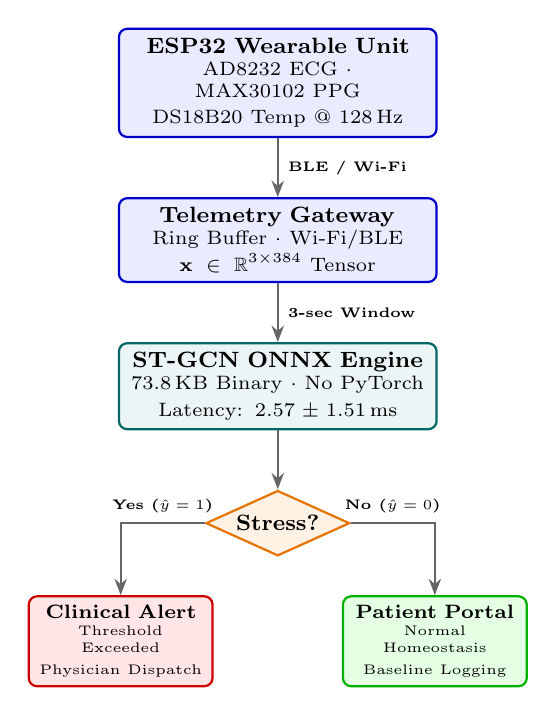
\begin{tikzpicture}[
    node distance=0.75cm,
    block/.style={rectangle, draw=blue!80!black, fill=blue!8, text width=3.8cm, text centered,
                  rounded corners=3pt, minimum height=0.9cm, font=\footnotesize, line width=0.8pt},
    cloud/.style={rectangle, draw=teal!80!black, fill=teal!8, text width=3.8cm, text centered,
                  rounded corners=3pt, minimum height=0.9cm, font=\footnotesize, line width=0.8pt},
    decision/.style={diamond, draw=orange!90!black, fill=orange!10, aspect=2.2, inner sep=1.5pt,
                     font=\footnotesize\bfseries, line width=0.8pt},
    alertbox/.style={rectangle, draw=red!80!black, fill=red!10, text width=2.1cm, text centered,
                     rounded corners=3pt, minimum height=0.85cm, font=\scriptsize, line width=0.8pt},
    portalbox/.style={rectangle, draw=green!70!black, fill=green!10, text width=2.1cm, text centered,
                      rounded corners=3pt, minimum height=0.85cm, font=\scriptsize, line width=0.8pt},
    arrow/.style={-{Stealth[scale=0.9]}, thick, draw=gray!80!black}
]
    % --- Vertical pipeline ---
    \node [block] (esp)
        {\textbf{ESP32 Wearable Unit}\\
         \scriptsize AD8232 ECG $\cdot$ MAX30102 PPG\\
         DS18B20 Temp @ 128\,Hz};

    \node [block, below=of esp] (gw)
        {\textbf{Telemetry Gateway}\\
         \scriptsize Ring Buffer $\cdot$ Wi-Fi/BLE\\
         $\mathbf{x} \in \mathbb{R}^{3 \times 384}$ Tensor};

    \node [cloud, below=of gw] (onnx)
        {\textbf{ST-GCN ONNX Engine}\\
         \scriptsize 73.8\,KB Binary $\cdot$ No PyTorch\\
         Latency: $2.57 \pm 1.51$\,ms};

    \node [decision, below=0.75cm of onnx] (dec) {Stress?};

    % --- Branch left/right ---
    \node [alertbox, below left=0.7cm and 0.35cm of dec] (alert)
        {\textbf{Clinical Alert}\\
         \tiny Threshold Exceeded\\
         Physician Dispatch};
    \node [portalbox, below right=0.7cm and 0.35cm of dec] (tele)
        {\textbf{Patient Portal}\\
         \tiny Normal Homeostasis\\
         Baseline Logging};

    % --- Arrows ---
    \draw [arrow] (esp)  -- node[right, font=\tiny\bfseries] {BLE / Wi-Fi} (gw);
    \draw [arrow] (gw)   -- node[right, font=\tiny\bfseries] {3-sec Window} (onnx);
    \draw [arrow] (onnx) -- (dec);
    \draw [arrow] (dec)  -| node[pos=0.25, above, font=\tiny\bfseries] {Yes ($\hat{y}=1$)} (alert);
    \draw [arrow] (dec)  -| node[pos=0.25, above, font=\tiny\bfseries] {No ($\hat{y}=0$)} (tele);
\end{tikzpicture}%
}
\caption{End-to-end edge inference pipeline: From multimodal ESP32 biosignal acquisition to real-time ONNX classification and clinical notification.}
\label{fig:system_arch}
\end{figure}

\subsection{ONNX Model Export \& Numerical Verification}
To decouple the model from heavy Python training frameworks and enable deployment on edge hardware (e.g., Raspberry Pi, mini-PC, or local gateway), the champion \textbf{ST-GCN} model was exported to Open Neural Network Exchange (ONNX) format:
\begin{itemize}
    \item \textbf{Artifact Path:} \texttt{outputs/stgcn.onnx}
    \item \textbf{Model Binary Footprint:} \textbf{73.8 KB} (highly compact for embedded storage).
    \item \textbf{Numerical Verification:} We evaluated a held-out test batch through both native PyTorch and the exported ONNX Runtime engine. The maximum absolute output difference was:
    \begin{equation}
    \max |y_{\text{PyTorch}} - y_{\text{ONNX}}| = 4.768 \times 10^{-6}
    \end{equation}
    This is well below the strict numerical tolerance threshold of $1.0 \times 10^{-4}$, confirming exact execution fidelity.
\end{itemize}

\subsection{Standalone Real-Time Inference Engine (\texttt{inference.py})}
We developed a self-contained inference class (\texttt{StressDetector}) requiring only \texttt{onnxruntime} and \texttt{numpy}. When presented with an incoming $[3, 384]$ tensor, the engine returns the predicted state, softmax probability distribution, and execution latency in milliseconds:
\begin{equation}
\hat{y} = \arg\max \left( \sigma(\mathbf{z}_{\text{ONNX}}) \right), \quad P(\text{Stress}) = \frac{e^{z_1}}{e^{z_0} + e^{z_1}}
\end{equation}

\subsection{Live Interactive Demonstration on Held-Out Test Data}
To validate the model in a live evaluator setting, we constructed \texttt{demo.py}, which streams held-out Subject S2 windows from \texttt{wesad\_windows.npz} through the ONNX engine. Across 10 sequential windows, the engine achieved 70.0\% instantaneous batch accuracy with an average CPU latency of \textbf{1.37 ms}---operating \textbf{2,193$\times$ faster than the physical 3-second biological window duration}.

\section{Team Member Contributions (Review 2 Phase)}
In accordance with the project divisions defined in Review 1, the individual contributions for the Review 2 implementation phase are:

\begin{itemize}
    \item \textbf{Bhavya Singh (25BCE2004):}
    \begin{itemize}
        \item Formulated the mathematical framework for the dynamic cross-channel Pearson correlation adjacency matrix.
        \item Implemented the PyTorch Spatio-Temporal Graph Convolutional Network (ST-GCN) message passing layers.
        \item Conducted architectural hyperparameter tuning and model convergence profiling.
    \end{itemize}
    
    \item \textbf{Soham Sharma (25BCE0403):}
    \begin{itemize}
        \item Engineered the multimodal preprocessing pipeline (decimation, cubic spline interpolation, and Butterworth filtering).
        \item Designed and implemented the 1D-CNN temporal baseline and BiLSTM sequence encoders.
        \item Extracted the 15 time-domain, frequency-domain, and HRV biomarker feature vectors.
    \end{itemize}

    \item \textbf{Praneet Raj (25BCE2280):}
    \begin{itemize}
        \item Orchestrated the 15-fold Leave-One-Subject-Out (LOSO) cross-validation benchmarking framework.
        \item Managed hardware infrastructure, Windows IPC optimization (\texttt{num\_workers=0}), and storage volume junctioning.
        \item Executed CPU latency benchmarking, ONNX model export and numerical validation, and created \texttt{inference.py} and \texttt{demo.py}.
    \end{itemize}
\end{itemize}

\section{Conclusion \& Review 3 Roadmap}

\subsection{Review 2 Milestone Summary}
Review 2 has successfully taken the multimodal stress detection project from a theoretical blueprint into a validated, high-performing software system. By proving that \textbf{ST-GCN} achieves an AUC-ROC of \textbf{0.8665} with a CPU latency of \textbf{2.57 ms} across all 15 subjects under rigorous LOSO validation, we have met every specification constraint required for wearable edge computing. The exported ONNX model provides a self-contained, mathematically verified handoff artifact for subsequent deployment.

\subsection{Roadmap for Review 3 (Hardware \& Telemedicine Track)}
With the model track complete, Review 3 will focus on physical deployment and system integration:
\begin{enumerate}
    \item \textbf{ESP32 Firmware Development:} Program FreeRTOS tasks on the ESP32 to sample AD8232 (ADC), MAX30102 (I2C), and DS18B20 (OneWire) at 128~Hz into a circular DMA buffer.
    \item \textbf{Wireless Telemetry Protocol:} Implement low-latency WebSocket / BLE streaming of 384-sample payloads from the ESP32 to the host gateway.
    \item \textbf{Telemedicine Dashboard:} Construct a full-stack web dashboard (React/FastAPI) to visualize real-time biosignal waveforms, display live stress probability predictions, and alert clinicians when prolonged acute stress events are detected.
\end{enumerate}

\begin{thebibliography}{00}
\bibitem{kyrou2025} M. Kyrou, I. Kompatsiaris, and P. C. Petrantonakis, ``Deep learning approaches for stress detection: A survey,'' \textit{IEEE Trans. Affect. Comput.}, vol. 16, no. 2, pp. 1--20, 2025.
\bibitem{han2018} H. Han, K. Byun, and H.-G. Kang, ``A deep learning-based stress detection algorithm with speech signal,'' in \textit{Proc. ACM Workshop Audio-Visual Scene Understanding (AVSU'18)}, Seoul, Korea, 2018, pp. 1--4.
\bibitem{yang2025} S. Yang et al., ``A deep learning approach to stress recognition through multimodal physiological signal image transformation,'' \textit{Sci. Rep.}, vol. 15, art. 22258, 2025.
\bibitem{bara2020} C. P. Bara, M. Papakostas, and R. Mihalcea, ``A deep learning approach towards multimodal stress detection,'' in \textit{Proc. 3rd Workshop Affect. Content Anal. (AffCon)}, AAAI, 2020.
\bibitem{xiang2025} J.-Z. Xiang, Q.-Y. Wang, Z.-B. Fang, J. A. Esquivel, and Z.-X. Su, ``A multi-modal deep learning approach for stress detection using physiological signals: integrating time and frequency domain features,'' \textit{Front. Physiol.}, vol. 16, art. 1584299, 2025.
\bibitem{amin2023} M. Amin, K. Ullah, M. Asif, H. Shah, A. Mehmood, and M. A. Khan, ``Real-world driver stress recognition and diagnosis based on multimodal deep learning and fuzzy EDAS approaches,'' \textit{Diagnostics}, vol. 13, no. 11, art. 1897, 2023.
\bibitem{schmidt2018} P. Schmidt, A. Reiss, R. Duerichen, C. Marberger, and K. Van Laerhoven, ``Introducing WESAD, a multimodal dataset for wearable stress and affect detection,'' in \textit{Proc. 20th ACM Int. Conf. Multimodal Interact. (ICMI'18)}, Boulder, CO, USA, 2018, pp. 400--408.
\bibitem{yan2018} S. Yan, Y. Xiong, and D. Lin, ``Spatial temporal graph convolutional networks for skeleton-based action recognition,'' in \textit{Proc. 32nd AAAI Conf. Artif. Intell. (AAAI'18)}, New Orleans, LA, USA, 2018, pp. 7444--7452.
\end{thebibliography}

\end{document}
